\documentclass{standalone}
\usepackage{tikz}
\usepackage{ctex,siunitx}
\usepackage{tkz-euclide}
\usepackage{amsmath}
\usetikzlibrary{patterns, calc}
\usetikzlibrary {decorations.pathmorphing, decorations.pathreplacing, decorations.shapes,}
\begin{document}
\small
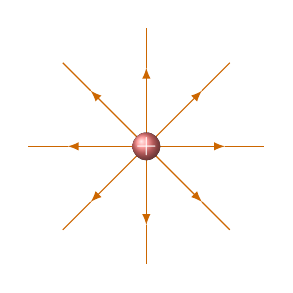
\begin{tikzpicture}[>=latex,scale=1.0]
  \foreach \x in {0,45,90,...,315}
	{
		\draw [orange!80!black,->](0:0)--(\x: 1.0);
		\draw [orange!80!black](\x:1.0)--(\x: 1.5);
	}
	\fill (0,0) [ball color=red!50] circle (5pt)node[text=white]{$+$};
\end{tikzpicture}
\end{document}